\documentclass[t, notes, xcolor=table]{beamer}

\usepackage{wrapfig}
\usepackage{float}
% For tabs in verbatim
\usepackage{fancyvrb}

% Adjust position of the image
\usepackage[export]{adjustbox}

% set fonts
\usefonttheme{professionalfonts} % using non standard fonts for beamer
\usepackage{txfonts,mathptmx}

% set indend spacing for first and second level indentation
\setlength{\leftmargini}{0.5cm}
\setlength{\leftmarginii}{0.5cm}
\setlength{\leftmarginiii}{0.5cm}

% Set circles for bullets 
\setbeamertemplate{itemize items}[circle]

% colors
\usepackage{xcolor}

% multiple columns
\usepackage{multicol}

% todo lists
\usepackage{pifont}
\usepackage{amssymb}

% increase space between text and frame name
\addtobeamertemplate{frametitle}{}{\vspace{0.5em}}

%Information to be included in the title page:
\title{Using Verilog Operators}
\author{Nikola Petrovic}
\institute{University of Belgrade, School of Electrical Engineering}
\date{2022}



\begin{document}

\frame{\titlepage}

%%%%%%%%%%%%%%%%%%%%%%%%%%%%%%%%%%%%%%%%%%%%%%%%%%%%%%%%%%%%
\begin{frame}
\frametitle{Module Objective}

In this module we will choose and use the Verilog operators correctly.

\begin{figure}[H!]
    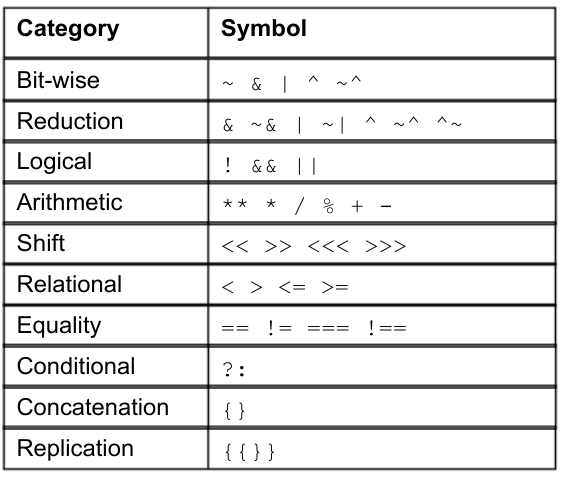
\includegraphics[width=0.5\textwidth]{img/05_operators.png}
\end{figure}

\end{frame}

%%%%%%%%%%%%%%%%%%%%%%%%%%%%%%%%%%%%%%%%%%%%%%%%%%%%%%%%%%%%
\begin{frame}[fragile]
\frametitle{Bit-Wise Operators}
\scriptsize{
\begin{multicols}{2}
\begin{itemize}
\item Bit-wise operators operate on vectors
\item Operations are performed bit by bit on individual bits
\item Unknown bits in an operand do not necessarily lead to unknown bits in result
\end{itemize}
\vfill
\begin{Verbatim}[commandchars=\\\{\}, tabsize=2]
\textcolor{purple}{not  ~}
\textcolor{purple}{and  &}
\textcolor{purple}{or   |}
\textcolor{purple}{xor  ^}
\textcolor{purple}{xnor ~^}
\textcolor{purple}{xnor ^~}
\end{Verbatim}

\columnbreak
\begin{figure}
    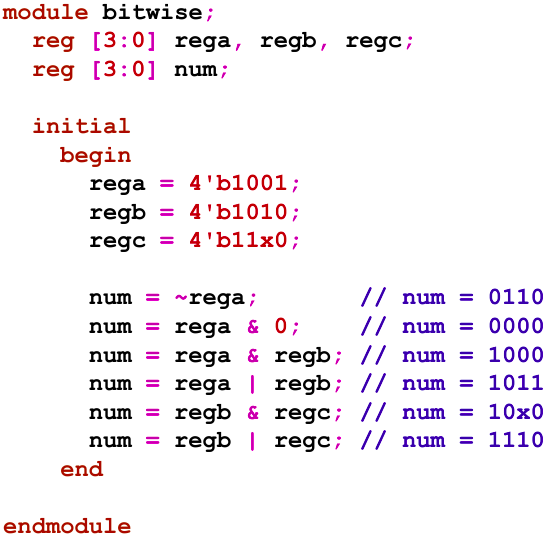
\includegraphics[width=0.45\textwidth]{img/05_bitwise.png}
\end{figure}
\end{multicols}
}
\end{frame}

\note{
\scriptsize{
The bitwise operators perform logical operations in a bitwise manner.
\newline

The bitwise unary negation operator inverts the logical sense of each bit of its operand. Each 0 becomes 1 and each 1 becomes 0, and each high-impedance bit becomes unknown.
\newline

The bitwise binary operators first zero-extend a smaller operand to match the width of a larger operand, and them perform logical operations on individual bit positions. Depending upon the operation, bits in one operand that are 0 or 1 can mask bits in the same position of the other operand that are high-impedance or unknown, so unknown bits in an operand do not necessarily produce unknown bits in the result.

}
}
%%%%%%%%%%%%%%%%%%%%%%%%%%%%%%%%%%%%%%%%%%%%%%%%%%%%%%%%%%%%
\begin{frame}[fragile]
\frametitle{Unary Reduction Operators}
\scriptsize{
\begin{multicols}{2}
\begin{itemize}
\item Reduction operators perform a bit-wise operation on all the bits of a single operand.
\item The result is always \verb+1'b0+, \verb+1'b1+ or \verb+1'bX+  
\end{itemize}
\vfill
\begin{Verbatim}[commandchars=\\\{\}, tabsize=2]
\textcolor{purple}{and  &}
\textcolor{purple}{or   |}
\textcolor{purple}{xor  ^}
\textcolor{purple}{nand ~&}
\textcolor{purple}{nor  ~|}
\textcolor{purple}{xnor ~^}
\textcolor{purple}{xnor ^~}
\end{Verbatim}

\columnbreak
\begin{figure}
    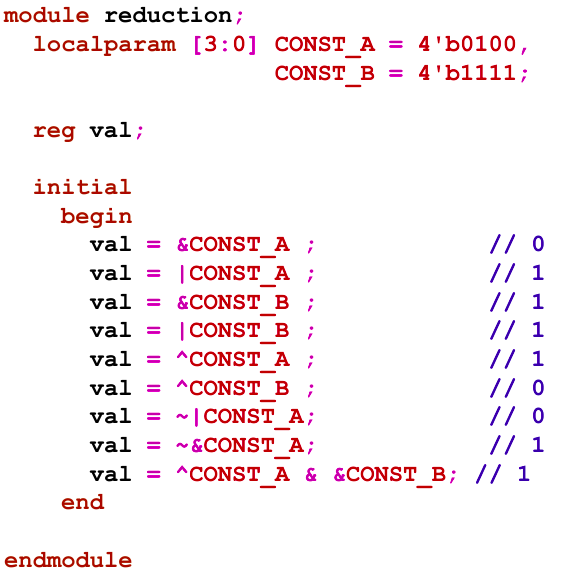
\includegraphics[width=0.45\textwidth]{img/05_reduction.png}
\end{figure}
\end{multicols}
}
\end{frame}
\note{
\footnotesize{
Unary reduction operators operate on all bits of a single operand to produce a single-bit result. The effect is as if the first applied the logical operation to the first two bits of the operand, then iteratively applied the logical operation to the current partial result and the next bit. The result of the operation is always a single bit that is 0, 1 or unknown (x).
\newline

We will see these same operators also used as bitwise binary operators. When used with single operand, they are reduction operators.

}
}

%%%%%%%%%%%%%%%%%%%%%%%%%%%%%%%%%%%%%%%%%%%%%%%%%%%%%%%%%%%%
\begin{frame}[fragile]
\frametitle{Logical Operators}
\scriptsize{
\begin{multicols}{2}
Logical operators interpret their operands as either true (1'b1), false (1'b0) or unknown (1'bX):
\begin{itemize}
\item 0: If all bits 0
\item 1: If any bit 1
\item X: If any bit is X or Z and no bits are 1
\end{itemize}
\vspace{6pt}
\begin{Verbatim}[commandchars=\\\{\}, tabsize=2]
\textcolor{purple}{not !}
\textcolor{purple}{and &&}
\textcolor{purple}{or  ||}
\end{Verbatim}
\vfill
\columnbreak
\begin{figure}
    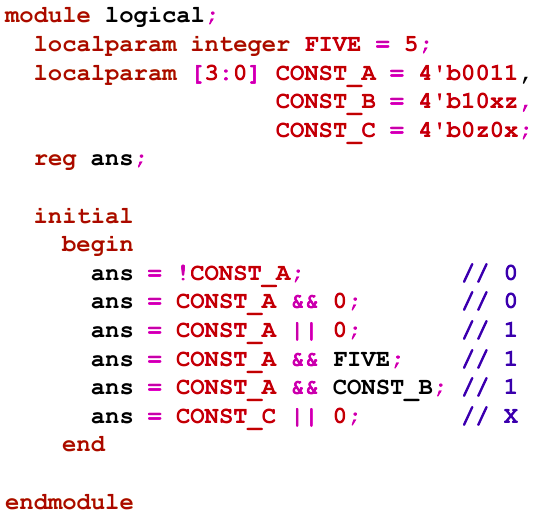
\includegraphics[width=0.45\textwidth]{img/05_logical.png}
\end{figure}
\end{multicols}
}
\end{frame}
\note{
\scriptsize{
Logical operators reduce each operand to a single bit, and then perform a single bit operation.
\newline

The rules for reduction of an operand are as follows:
\begin{itemize}
\item If the operand contains all zeroes, it reduces to logic 0.
\item If the operand contains any ones, it reduces to logic 1.
\item If the operand contain no ones, but does contain one or more high-impedance or unknown values, it reduces to unknown, because its logical values is unknown.
\end{itemize}

The unary logical negation operator then inverts the logical sense of its operand. 0 becomes 1, and 1 becomes 0.
\newline

The binary conjunction  and disjunction operators produce the logical conjunction and disjunction respectively, of their operands.
\newline

\textbf{Design Tip:} Generally, logical operators should be avoided unless explicitly required. It is very easy to get into the habit of using logical operators everywhere. They are identical to bitwise operators for single bit expressions, but give very  results when using vectors.

}
}


%%%%%%%%%%%%%%%%%%%%%%%%%%%%%%%%%%%%%%%%%%%%%%%%%%%%%%%%%%%%
\begin{frame}
\frametitle{Arithmetic Operators}
\scriptsize{
\begin{multicols}{2}
Verilog-1995:
\begin{itemize}
\item Add +
\item Subtract -
\item Multiply *
\item Divide /
\item Modulus \%
\item Unsigned: base literal, net, \textbf{reg}, \textbf{time}
\item Signed: unbased literal, \textbf{integer}
\end{itemize}
Verilog-2001:
\begin{itemize}
\item Exponential Power **
\end{itemize}
\vfill
\columnbreak
\begin{figure}
    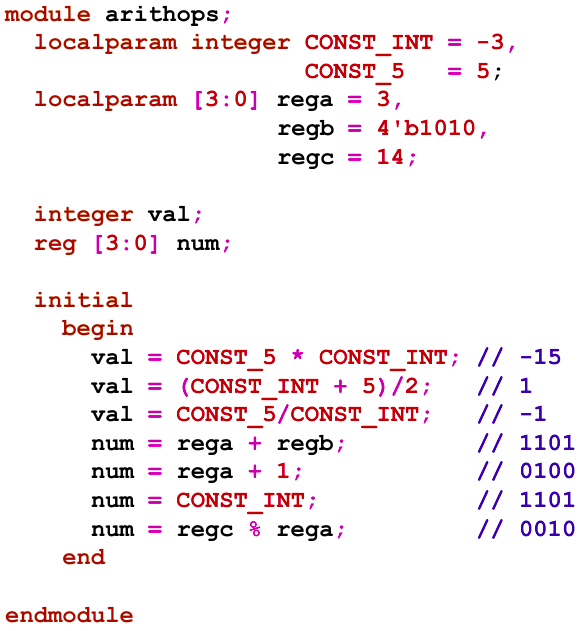
\includegraphics[width=0.45\textwidth]{img/05_arith.png}
\end{figure}
\end{multicols}
}
\end{frame}
\note{
\scriptsize{
The Verilog-1995 arithmetic operators are add, subtract, multiply, divide and modulus. Verilog-2001 added the power operator.
\newline

This example declares two \textit{integer} parameters, three 4-bit vector \textit{reg} parameters, an \textit{integer} variable and a 4-bit vector \textit{reg} variable, and performs some operations with them. See where integer division discards the fractional part. See where assigning 3 to an unsigned 4-bit vector \textit{reg} keeps the same rightmost four bits but now interprets the value as +13.
\newline

Some additional information about arithmetic operators:
\begin{itemize}
\item Any Z or X bit in either operand produces an unknown (X) result.
\item Integer division discards any remaining fractional part.
\item Division or modulo by 0 produces an unknown (X) result.
\item Raising 0 to a negative power produces an  result.
\item Raising a negative value to a real power produces an unspecified result. 
\end{itemize}

}
}

%%%%%%%%%%%%%%%%%%%%%%%%%%%%%%%%%%%%%%%%%%%%%%%%%%%%%%%%%%%%
\begin{frame}
\frametitle{Enhanced Signed Arithmetic}

\textbf{Verilog-2001}: New reserved word: \textbf{signed}
\begin{itemize}
\item \textcolor{purple}{signed} keyword treats literal, function, net, reg as signed
\item Arithmetic right shift operators maintains the sign of a value
\item \textcolor{purple}{\$signed} and \textcolor{purple}{\$unsigned} system functions cast value
\end{itemize}

\begin{figure}
    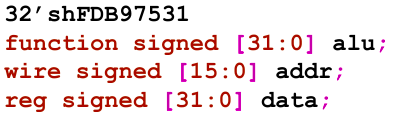
\includegraphics[width=0.45\textwidth]{img/05_enhanced.png}
\end{figure}
\end{frame}
\note{
\scriptsize{
The parser interprets an integer with no base specified as a signed value in 2's complement form: 

intA = -12/3;
\begin{itemize}
\item The left operand is a 32-bit signed value 12, negated
\item The expression result is -4
\end{itemize}
The parser interprets an integer with an unsigned base specifier as an unsigned value:

intA = -'\textbf{d}12/3;
\begin{itemize}
\item The left operand is a 32-bit unsigned value 12, negated.
\item The expression result is 1431655761
\end{itemize}
The parser interprets an integer with an signed base specifier as an signed value: 

intA = -4'\textbf{sd}12/3;
\begin{itemize}
\item The left operand is a 4-bit pattern of 12 (1100) interpreted as a signed number (-4) and then negated (4)
\item The expression result is 1
\end{itemize}

}
}

%%%%%%%%%%%%%%%%%%%%%%%%%%%%%%%%%%%%%%%%%%%%%%%%%%%%%%%%%%%%
\begin{frame}
\frametitle{Signed Vectors}

\end{frame}

%%%%%%%%%%%%%%%%%%%%%%%%%%%%%%%%%%%%%%%%%%%%%%%%%%%%%%%%%%%%
\begin{frame}
\frametitle{Module}

\end{frame}

%%%%%%%%%%%%%%%%%%%%%%%%%%%%%%%%%%%%%%%%%%%%%%%%%%%%%%%%%%%%
\begin{frame}
\frametitle{Module}

\end{frame}

%%%%%%%%%%%%%%%%%%%%%%%%%%%%%%%%%%%%%%%%%%%%%%%%%%%%%%%%%%%%
\begin{frame}
\frametitle{Module}

\end{frame}

%%%%%%%%%%%%%%%%%%%%%%%%%%%%%%%%%%%%%%%%%%%%%%%%%%%%%%%%%%%%
\begin{frame}
\frametitle{Module}

\end{frame}

%%%%%%%%%%%%%%%%%%%%%%%%%%%%%%%%%%%%%%%%%%%%%%%%%%%%%%%%%%%%
\begin{frame}
\frametitle{Module}

\end{frame}

%%%%%%%%%%%%%%%%%%%%%%%%%%%%%%%%%%%%%%%%%%%%%%%%%%%%%%%%%%%%
\begin{frame}
\frametitle{Module}

\end{frame}

%%%%%%%%%%%%%%%%%%%%%%%%%%%%%%%%%%%%%%%%%%%%%%%%%%%%%%%%%%%%
\begin{frame}
\frametitle{Module}

\end{frame}

%%%%%%%%%%%%%%%%%%%%%%%%%%%%%%%%%%%%%%%%%%%%%%%%%%%%%%%%%%%%
\begin{frame}
\frametitle{Module}

\end{frame}

%%%%%%%%%%%%%%%%%%%%%%%%%%%%%%%%%%%%%%%%%%%%%%%%%%%%%%%%%%%%
\begin{frame}
\frametitle{Module}

\end{frame}

\end{document}
